\documentclass[12pt,a4paper]{article}
\usepackage[utf8]{inputenc}
\usepackage[english]{babel}
\usepackage{amsmath}
\usepackage{amsfonts}
\usepackage{amssymb}
\usepackage{graphicx}
\usepackage[left=2cm,right=2cm,top=2cm,bottom=2cm]{geometry}
\begin{document}

\raggedright

\section*{Questionnaire 2}

\begin{enumerate}
\item Provide an example of where the bear classification model might work poorly in production, due to structural or style differences in the training data. \\

\smallbreak

There are many cases that the bear classification model could fail, especially if these cases were not represented in the training data:
\begin{itemize}
\item The bear is partially obstructed
\item Nighttime images are passed into the model
\item Low-res images are passed into the model
\item The bear is far away from the camera
\item The bear training dataset is highly biased toward one type of feature (i.e., color)
\end{itemize}

\bigbreak

\item Where do text models currently have a major deficiency? \\

\smallbreak

Text models can generate appropriate text (like replies or imitating author style); however, text models still struggle with generating \textit{correct} responses. Given factual information (such as a knowledge base), it is still hard to generate responses that utilizes this information to generate factually correct responses, though this text can seem very compelling. This can be very dangerous, because people unfamiliar with the subject may not be able to evaluate the factual accuracy of the generated text.

\bigbreak

\item What are possible negative societal implications of text generation models? \\

\smallbreak

The ability for text generation models to generate context-aware, highly compelling responses can be used at a massive scale to spread disinformation and encourage conflict. \\
\smallbreak
Models also reinforce bias (like gender or racial bias) in training data and can create a vicious cycle of biased outputs.

\bigbreak

\item In situations where a model might make mistakes, and those mistakes could be harmful, what is a good alternative to automating a process? \\

\smallbreak

The prediction could then be reviewed by a human professional, who can determine whether the prediction was accurate or not. For example, a machine learning model for identifying strokes in CT scans can alert high priority cases for expedited review, while other cases can be sent to radiologist for regular review. \\
\smallbreak
Other models can also augment a medical professional's abilities, reducing risk but improving efficiency of the workflow. For example, deep learning models can provide useful measurements for radiologists or pathologists.

\bigbreak

\item What kind of tabular data is deep learning particularly good at? \\

\smallbreak

Deep learning is good at analyzing tabular data that includes natural language, or high cardinality categorical items (containing larger number of discrete choices like zip code).

\bigbreak

\item What's a key downside of directly using a deep learning model for recommendation systems? \\

\smallbreak

Current (as of 2020) machine learning approaches for recommendation systems will only tell what products a user might like, and may not be recommendations that would be helpful to the user. For example, if a user if familiar with other books from the same author, it isn't helpful to recommend those products even though the user bought the author's book. 

\bigbreak

\item What are the steps of the Drivetrain Approach? \\

\smallbreak

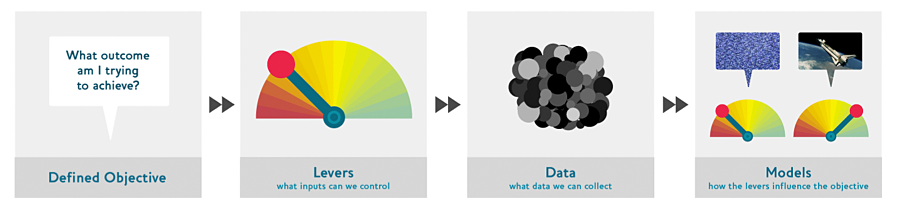
\includegraphics[scale=0.5]{drivetrain.png}

\bigbreak

\item How do the steps of the Drivetrain Approach map to a recommendation system? \\

\smallbreak

The \textbf{objective} of a recommendation engine is to drive additional sales by surprising and delighting the customer with recommendations of items they would not have purchased without the recommendation. The \textbf{lever} is the ranking of the recommendations. New \textbf{data} must be collected to generate recommendations that will cause new sales . This will require conducting many randomized experiments in order to collect data about a wide range of recommendations for a wide range of customers. This is a step that few organizations take; but without it, you don’t have the information you need to actually optimize recommendations based on your true objective (more sales!)

\bigbreak

\item Create an image recognition model using data you curate, and deploy it on the web. \\

Placeholder

\item What is \verb/DataLoaders/? \\

\smallbreak

The \verb/DataLoaders/ class is the class that passes the data to the fastai model. It is essentially a class that stores the required \verb/DataLoader/ objects (usually for train and validation sets).

\bigbreak

\item What four things do we need to tell fastai to create \verb/DataLoaders/? \\

\smallbreak

\begin{itemize}
\item what kinds of data we are working with
\item how to get the list of items
\item how to label these items
\item how to create the validation set
\end{itemize}

\bigbreak

\item What does the splitter parameter to \verb/DataBlock/ do? \\

\smallbreak

The splitter parameter is used as a way for fastai to split up the dataset into multiple subsets (usually train and validation sets). For example, to randomly split the data, you can use fastai's predefined \verb/RandomSplitter/ class, providing it with the proportion of the data used for validation.

\bigbreak

\item How do we ensure a random split always gives the same validation set? \\

\smallbreak

It turns out that it is impossible to create truly random numbers. Instead, computers use a process known as a pseudo-random generator. However, this process can be controlled using a random seed. By setting a seed value, the pseudo-random generator will generate the same "random" numbers in a fixed manner which will be the same for every run as long as the seed is the same. By using a random seed, we can generate a random split that always gives the same validation set.

\bigbreak

\item What letters are often used to signify the independent and dependent variables? \\

\smallbreak

x is independent. y is dependent.

\bigbreak

\item What's the difference between the \verb/crop/, \verb/pad/, and \verb/squish/ \verb/Resize()/ approaches? When might you choose one over the others? \\

\smallbreak

\begin{center}
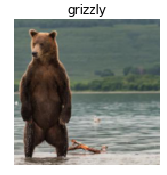
\includegraphics[scale=1]{crop_grizzly}
\end{center}

\verb/crop/ is the default \verb/Resize()/ method, and it \textit{crops} the images to fit the a square shape of the size requested, using the full width or height. \\
\smallbreak
In this case, this can result in losing some important details. For example, if we were trying to recognize the breed of dog or cat, we may end up cropping out a key part of the body or the face necessary to distinguish between similar breeds.

\begin{center}
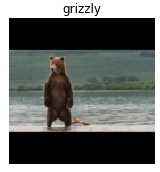
\includegraphics[scale=1]{pad_grizzly}
\end{center}

\verb/pad/ is an alternate \verb/Resize()/ method, which pads the matrix of the image's pixels with zeros (which shows as black when viewing the images). \\

\begin{center}
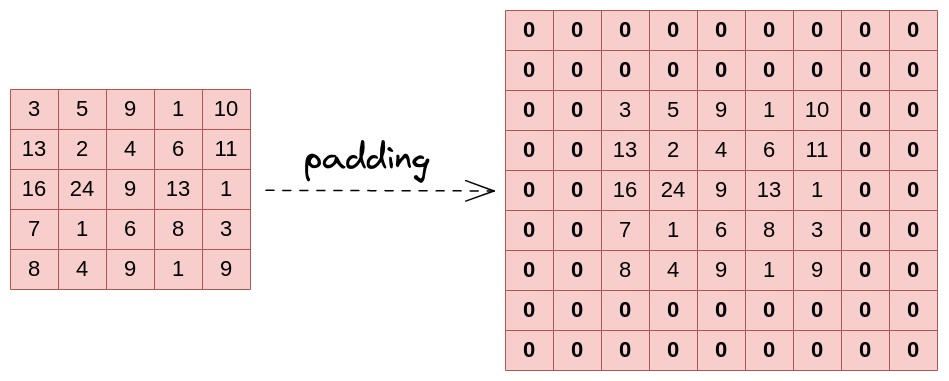
\includegraphics[scale=0.5]{padding.png}
\end{center}

For convolutional networks, the center pixels are much more relevant than corner pixels, which are employed less often and are not as involved when applying a convolutional operation to a matrix. This causes the edges of the \textbf{input} picture to lose relevant information. Padding attempts to solve this issue. \\
\smallbreak
In this case, padding images results in a lot of empty space, which results in a lower effective resolution for the part of the image we actually use.

\begin{center}
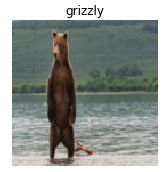
\includegraphics[scale=1]{squish_grizzly.png}
\end{center}

\verb/squish/ is another alternative \verb/Resize()/ method, which can either squish or stretch the image. This can cause the image to take on an unrealistic shape, leading to a model that learns that things look different to how they actually are, which we would expect to result in lower accuracy.

\bigbreak

Which resizing method to use therefore depends on the underlying problem and dataset. For example, if the features in the dataset images take up the entire image and cropping may result in loss of information, then padding or squishing may be more suitable. \\
Another better method is \verb/RandomResizedCrop/, in which we crop on a randomly selected region of the image; during every epoch, the model will see a different part of the image and will learn accordingly. 

\bigbreak

\item What is data augmentation? Why is it needed? \\

\smallbreak

Data augmentation refers to creating random variations of our input data, such that they appear different, but not so different it changes the meaning of the data. Examples include flipping, rotation, perspective warping, brightness changes, etc. \\
\smallbreak
Data augmentation is useful for the model to better understand the basic concept of what an object is and how the objects of interest are represented in images. Therefore, data augmentation allows machine learning models to \textit{generalize}. This is especially important when it can be slow and expensive to label data, or when there is little data.

\bigbreak

\item What is the difference between \verb/item_tfms/ and \verb/batch_tfms/? \\

\smallbreak

\verb/item_tfms/ are transformations applied to a single data sample \verb/x/ on the CPU. \verb/Resize()/ is a common transform because the mini-batch of input images to a CNN must have the same dimensions. Assuming the images are RGB with 3 channels, then \verb/Resize()/ as \verb/item_tfms/ will make sure the images have the same width and height. \\
\smallbreak
\verb/batch_tfms/ are applied to batched data samples (aka individual samples that have been collated into a mini-batch) on the GPU. They are faster and more efficient than \verb/item_tfms/. A good example of these are the ones provided by \verb/aug_transforms()/. Inside are several batch-level augmentations that help many models. 
\item What is a confusion matrix? \\

\smallbreak

A class confusion matrix is a representation of the predictions made vs. the correct models. The rows of the matrix represent the actual labels while the columns represent the predictions. Therefore, the number of images in the diagonal elements represent the number of correctly classified images, while the off-diagonal elements are incorrectly classified images. Class confusion matrices provide useful information about how well the model is doing and which classes the model might \textit{confusing}.

\bigbreak

\item What does \verb/export/ save? \\

\smallbreak

\verb/export/ saves both the architecture, as well as the trained parameters of the neural network architecture. It also saves how the \verb/DataLoaders/ are defined.

\bigbreak

\item What is it called when we use a model for getting predictions, instead of training? \\

\smallbreak

Inference.

\bigbreak

\item What are IPython widgets? \\

\smallbreak

IPython widgets are JavaScript and Python combined functionalities that let us build and interact with GUI components directly in a Jupyter notebook. An example of this would be an upload button, which can be created with the Python function \verb/widgets.FileUpload()/.

\bigbreak

\item When might you want to use CPU for deployment? When might GPU be better? \\

\smallbreak

GPUs are best for doing identical work in parallel. If you will be analyzing single pieces of data at a time (like a single image or a single sentence), then CPUs may be more cost-effective instead, especially with more market competition for CPU servers vs. GPU servers. GPUs could be used if you collect user responses into a batch at a time, and perform inference on the batch. This may require the user to wait for model predictions. Additionally, there are many other complexities when it comes to GPU inference, like memory management and queuing of the batches.

\bigbreak

\item What are the downsides of deploying your app to a server, instead of to a client (or edge) device such as a phone or PC? \\

\smallbreak

The application will require a network connection, and there will be extra network latency time when submitting input and returning results. Additionally, sending private data to a network server can lead to security concerns. \\
\smallbreak
Conversely, deploying a model to a server makes it easier to iterate and roll out new versions of a model. This is because you, as a developer, have full control over the server environment and only need to do it once rather than having to make sure that all the endpoints (phones, PCs) upgrade their version individually.

\bigbreak

\item What are three examples of problems that could occur when rolling out a bear warning system in practice? \\

\smallbreak

The model I trained will likely perform poorly when:
\begin{itemize}
\item[1.] Handling nighttime images
\item[2.] Dealing with low-res images (ex: some smartphone images)
\item[3.] The model returns prediction too slowly to be useful
\end{itemize}

\bigbreak

\item What is "out-of-domain data"? \\

\smallbreak

Out-of-domain data is data that is fundamentally different in some aspect compared to the model's training data. For example, an object detector that was trained exclusively with outside daytime photos is given a photo taken at night.

\bigbreak

\item What is "domain shift"? \\

\smallbreak

This is when the type of data changes gradually over time. For example, an insurance company is using a deep learning model as part of their pricing algorithm, but over time their customers will be different, with the original training data not being representative of current data, and the deep learning model being applied on effectively out-of-domain data.

\bigbreak

\item What are the three steps in the deployment process? \\

\smallbreak

\begin{itemize}
\item[1.] Manual process -- The model is run in parallel and not directly driving any actions, with humans still checking the model outputs.
\item[2.] Limited scope deployment -- The model's scope is limited and carefully surprised. For example, doing a geographically and time-constrained trial of model deployment that is carefully supervised.
\item[3.] Gradual expansion -- The model scope is gradually increased, while good reporting systems are implemented in order to check for any significant changes to the actions taken compared to the manual process (i.e. the models should perform similarly to the humans, unless it is already anticipated to be better).
\end{itemize}

\end{enumerate}

\section*{Further Research}

\begin{enumerate}
\item Consider how the Drivetrain Approach maps to a project or problem you're interested in. \\

\smallbreak

A project that I'm interested in is classifying song genres from audio (from Datacamp).
\smallbreak
\textbf{Defined Objective}: The objective is to take audio data and attempt to interpret what genre the song belongs to.
\smallbreak
\textbf{Levers}: The lever is the ranking of the genres.
\smallbreak
\textbf{Data}: Data can be collected by visualizing the audio.

\bigbreak

\item When might it be best to avoid certain types of data augmentation? \\

\smallbreak

Some common data augmentation techniques for convolutional neural networks (CNN) are:
\begin{itemize}
\item[1.] Cropping \\
\smallbreak
Cropping might take out some important details of the image you are trying to input as training data.

\item[2.] Flipping \\
\smallbreak
Specific regions of an image may not always be interchangeable (e.g. vertical flipping a CT scan of lungs so that the left lung is on the right side and vice versa).

\item[3.] Scaling \\
\smallbreak
Typically, scaling up lowers image quality, which may make the image lose some features.

\item[4.] Brightness \\
\smallbreak
Any feature that is dependent on color may be affected negatively. It can cause the model to become confused (e.g. brightening a grizzly bear's fur can cause it to look brown and therefore be confused with a brown bear).

\item[5.] Color Augmentation \\
\smallbreak
Any feature that is dependent on color may be affected negatively.

\end{itemize}

\bigbreak

\item For a project you're interested in applying deep learning to, consider the thought experiment "What would happen if it went really, really well?" \\

\smallbreak

It would be really hard for a project like this to become really good because of numerous elements that comprise a single genre and the fact that new elements and genres themselves are being added every year. If, hypothetically, it did reach this level of competence, all music could easily be defined just based on this model. This will decrease the amount of genres there are since music would be more easily be categorized.
\end{enumerate}

\end{document}